%
% loesung.tex -- Beispiel-File für die Beschreibung der Loesung
%
% (c) 2020 Prof Dr Andreas Müller, Hochschule Rapperswil
%
\section{Anwendungen
\label{pade:section:Anwendungen}}
\rhead{Anwendungen}

In diesem Kapitel werden ein paar Anwendungsmöglichkeiten der Padé-Approximation gezeigt.



\subsection{Totzeit Approximation
\label{pade:subsection:totzeit}}

In der Elektrotechnik werden des öfteren mathematische Probleme im Frequenzbereich gelöst da dies oft einfacher ist.
Bei der Totzeit spricht man dabei von einer Verzögerung im Zeitbereich, welcher zum Beispiel in einem Regelkreis vorkommen kann.
Solche Lineare zeitinvariante Systeme (LZI) oder besser bekannt unter dem englischen Begriff linear time-invariant system (LTI), sind unabhängig von zeitlichen Verschiebungen. 
Jeder der sich mit LTI Systemen auseinander gesetzt hat weiss das eine Totzeit $T$ im Bildbereich
\begin{equation*}
H(s) = e^{-sT}
\end{equation*}
durch eine Exponentialfunktion ausgedrückt wird.
Die meisten Übertragungsfunktionen hingegen kommen als gebrochene Polynome, eine Form welche einer rationalen Funktion
\begin{equation*}
H(s)=\frac{P(s)}{Q(s)}
\end{equation*}
entspricht.
Diese gebrochenen Polynome verwendet man dann um Pol- und Nullstellen zu finden um damit dann weitere Analysen durchzuführen. 
Mit $e^{-sT}$ haben wir jedoch keine Polstellen welche wir Analysieren können.
Dies kann jedoch gefordert sein wenn man eine zeit kontinuierliche Analyse machen möchte.
Eine Lösung dafür könnte nun sein $e^{-sT}$ zu approximieren und die Approximation für die weiteren Rechnungen zu verwenden.
Die Padé-Approximation der Exponentialfunktion ist glücklicherweise schon sehr gut bekannt \cite{pade:moler}

\begin{equation}
R_{L, M}(x)
=
\frac{P_{L, M}(x)}{Q_{L, M}(x)} \approx e^{-x}
\end{equation}
wobei $P_{L, M}(x)$ das Zählerpolynom ist
\begin{equation}
P_{L, M}(x)
=
\sum_{j=0}^{L} \frac{(L+M-j) ! L !}{(L+M) ! j !(L-j) !}(-x)^{j}
\end{equation}
und $Q_{L, M}(x)$ das Nennerpolynom der Padéapproximation
\begin{equation}
Q_{L, M}(x)
=
\sum_{j=0}^{M} \frac{(L+M-j) ! M !}{(L+M) ! j !(M-j) !} x^{j}.
\end{equation}
Diesen beide Polynome können verwendet werden um die dazugehörige Padé-Liste 

\begin{equation}\begin{array}{lll}
R_{[1,1]}(x)=\frac{1-\frac{1}{2} x}{1+\frac{1}{2} x} & 
R_{[1,2]}(x)=\frac{1-\frac{1}{3} x}{1+\frac{2}{3} x+\frac{1}{6} x^{2}} & 
R_{[1,3]}(x)=\frac{1-\frac{1}{4} x}{1+\frac{3}{4} x+\frac{1}{4} x^{2}+\frac{1}{24} x^{3}} \\
R_{[2,1]}(x)=\frac{1-\frac{2}{3} x+\frac{1}{6} x^{2}}{1+\frac{1}{3} x} & 
R_{[2,2]}(x)=\frac{1-\frac{1}{2} x+\frac{1}{12} x^{2}}{1+\frac{1}{2} x+\frac{1}{12} x^{2}} &
R_{[2,3]}(x)=\frac{1-\frac{2}{5} x+\frac{1}{20} x^{2}}{1+\frac{3}{5} x+\frac{3}{20} x^{2}+\frac{1}{60} x^{3}} \\
R_{[3,1]}(x)=\frac{1-\frac{3}{4} x+\frac{1}{4} x^{2}-\frac{1}{24} x^{3}}{1+\frac{1}{4} x} &
R_{[3,2]}(x)=\frac{1-\frac{3}{5} x+\frac{3}{20} x^{2}-\frac{1}{60} x^{3}}{1+\frac{2}{5} x+\frac{1}{20} x^{2}} &
R_{[3,3]}(x)=\frac{1-\frac{1}{2} x+\frac{1}{10} x^{2}-\frac{1}{120} x^{3}}{1+\frac{1}{2} x+\frac{1}{10} x^{2}+\frac{1}{120} x^{3}}
\end{array}\end{equation}
zu berechnen.

In der Grafik \ref{pade:totzeitexp} ist ersichtlich das die Approximation mit steigendem Grad bessere Resultate liefert.
Die Grade werden dabei im Nenner und Zähler unterteilt aufgezeigt.
In diesem Beispiel mit der Exponentialfunktion erweisen sich die Polynome des selben Grades im Nenner und Zähler als die geeignetsten.
Wobei mit steigendem Grad eine stetige Verbesserung zugrunde liegt.
\begin{figure}
	\centering
	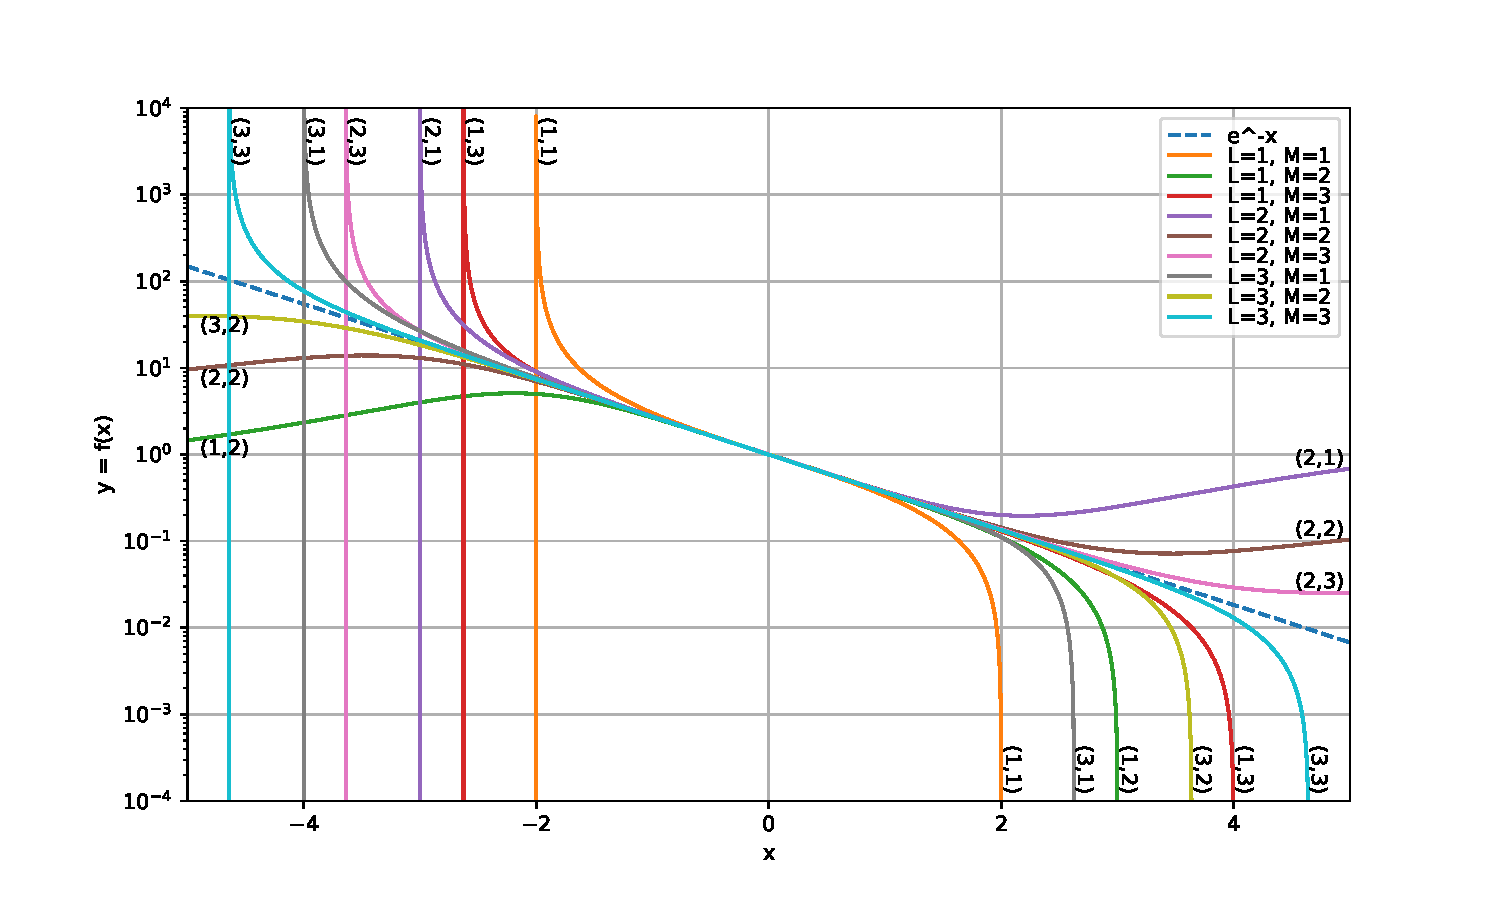
\includegraphics[width=1\linewidth]{./papers/pade/python/bilder/totzeit.pdf}
	\caption{Aufzeigen der Padé-Approximationen der Exponentialfunktion im Vergleich zu der Originalfunktion \label{pade:totzeitexp}}
\end{figure}

Nehmen wir nun diese Polynome und welche sich noch im Bildbereich befinden und transformieren diese wieder zurück in den Zeitbereich, erhalten wir die in der Grafik \ref{pade:totzeitexp2} Kurven.
\begin{figure}
	\centering
	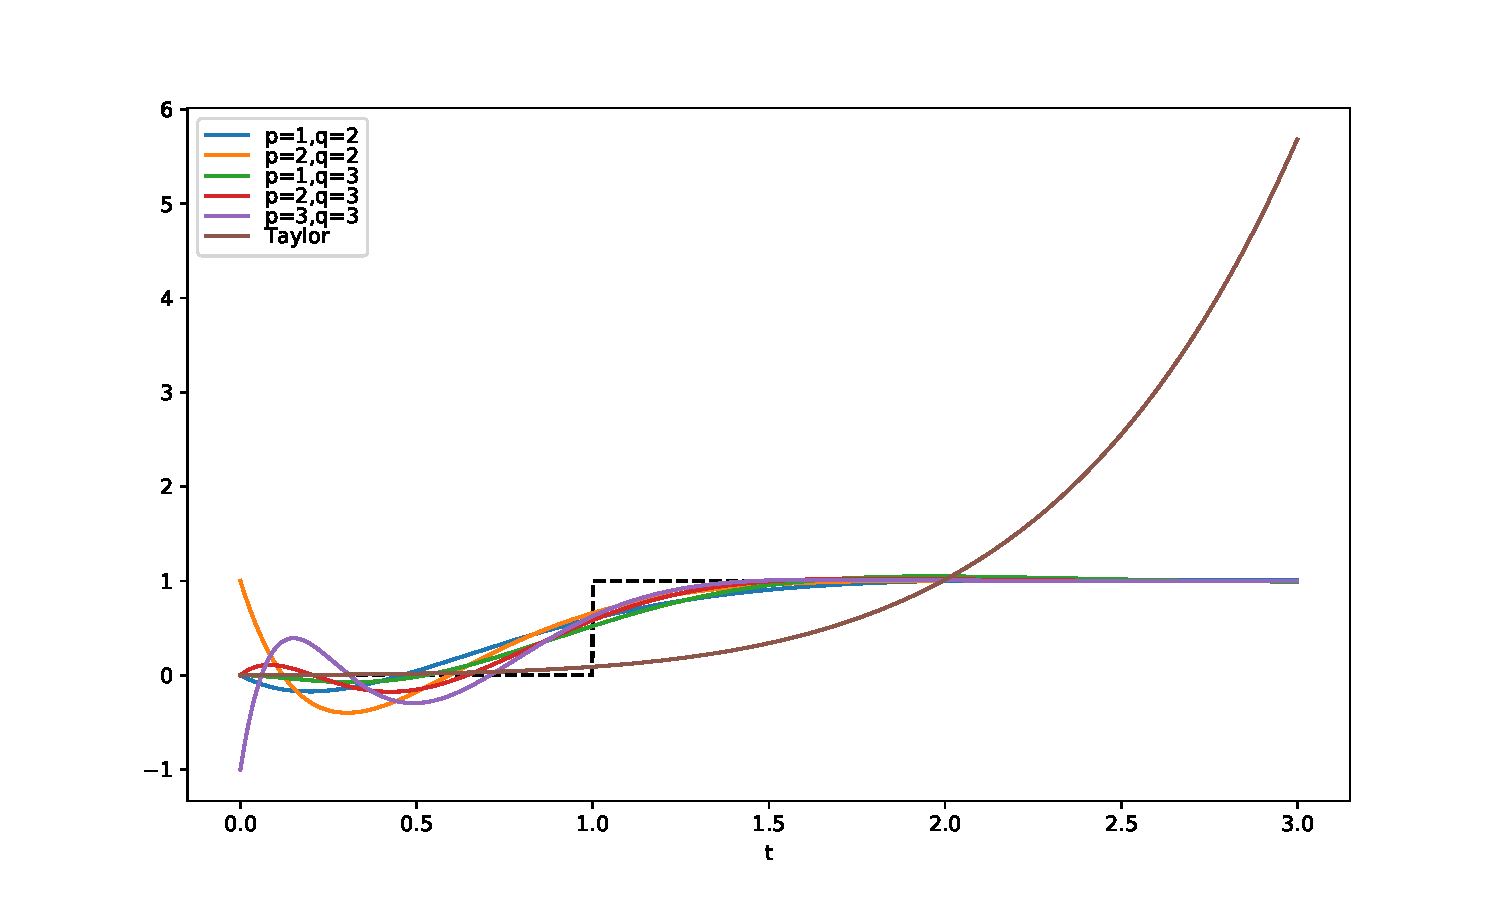
\includegraphics[width=1\linewidth]{./papers/pade/python/bilder/padelow33.pdf}
	\caption{In den Zeitbereich zurück transformierte Polynome tieferer Ordnung\label{pade:totzeitexp2}.}
\end{figure}

Die Polynome unterer Ordnung sind dabei noch weit von einem brauchbaren Ergebnis entfernt.
Man kann nun die Ordnung der Polynome weiter erhöhen bis man eine zufriedenstellende Approximation erhält.
Dabei muss man jedoch aufpassen welche Funktion für die Rücktransformation verwendet wird, da nicht alle Implementationen nummerisch stabil sind bei Polynomen grosser Ordnung.

\todo{Polstellen und Nullstellen erklären mit unstabilität}

\begin{figure}
	\centering
	\subfigure[Pole und Nullstellen im Bildbereich geplottet wenn $L=M$ ist.\label{pade:poles1}]{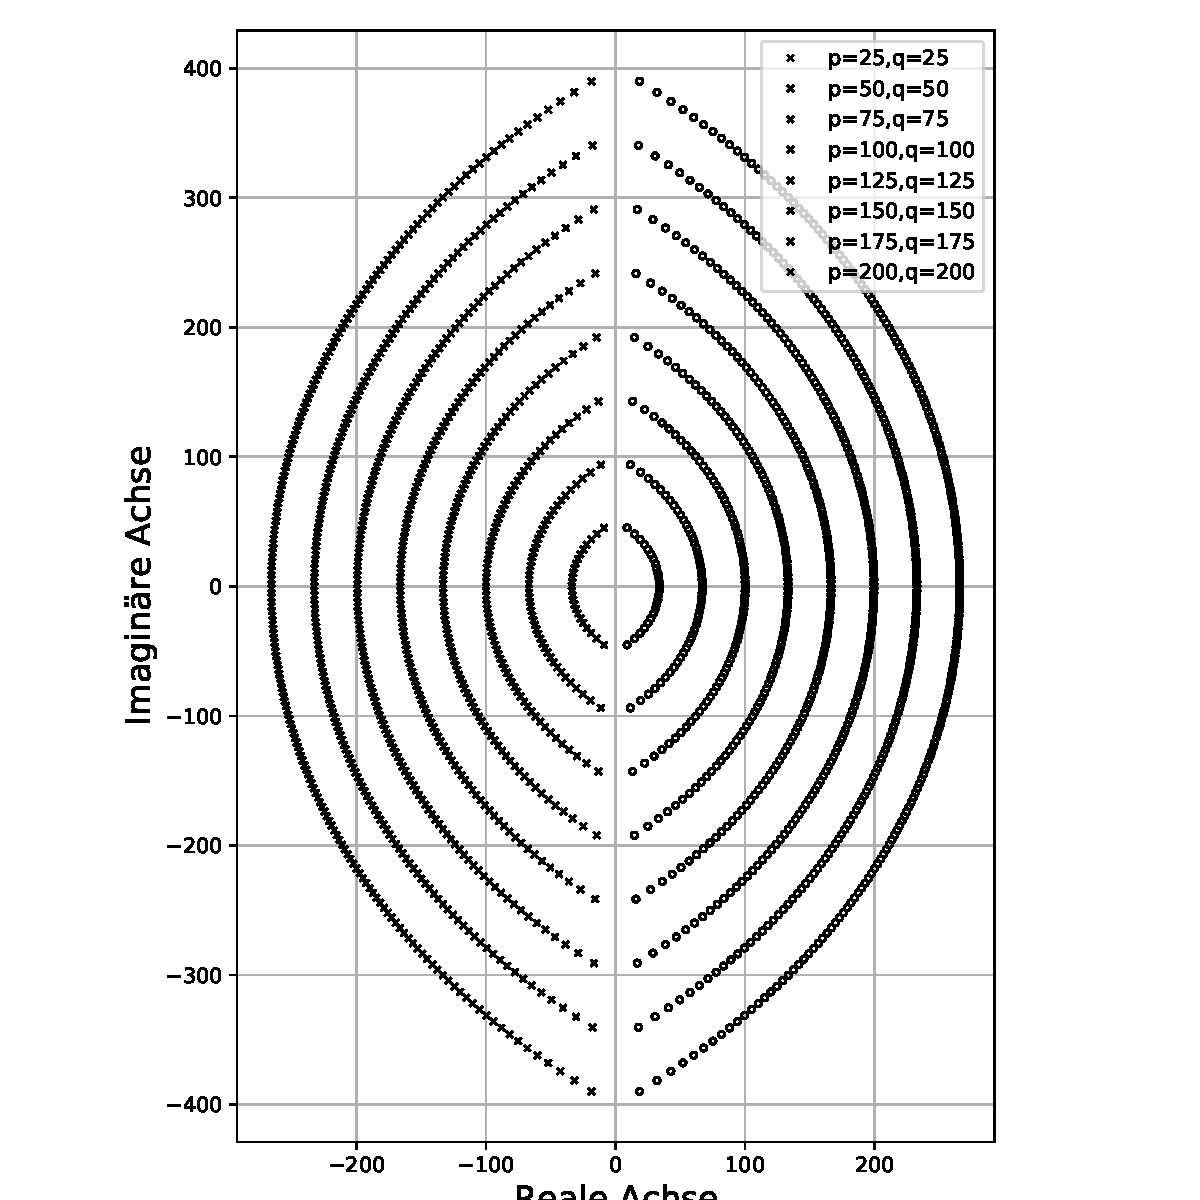
\includegraphics[width=0.50\linewidth]{./papers/pade/python/bilder/poles1.pdf}}
	\subfigure[Pole und Nullstellen im Bildbereich geplottet wenn $L>M$ ist.\label{pade:poles2}]{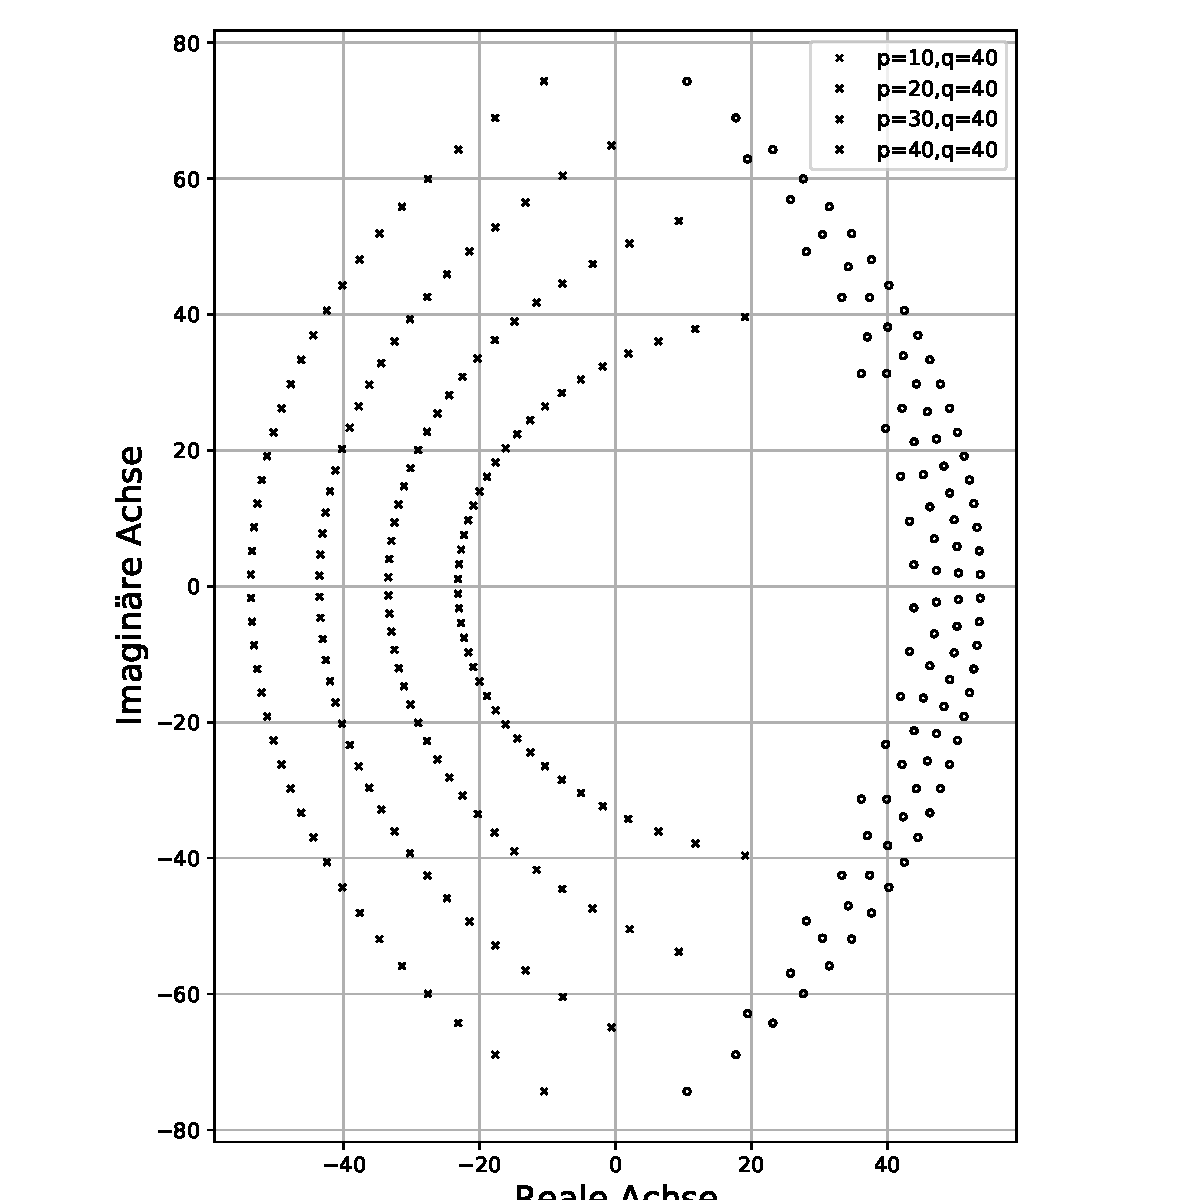
\includegraphics[width=0.45\linewidth]{./papers/pade/python/bilder/poles2.pdf}}
	\subfigure[Pole und Nullstellen im Bildbereich geplottet wenn $L<M$ ist.\label{pade:poles3}]{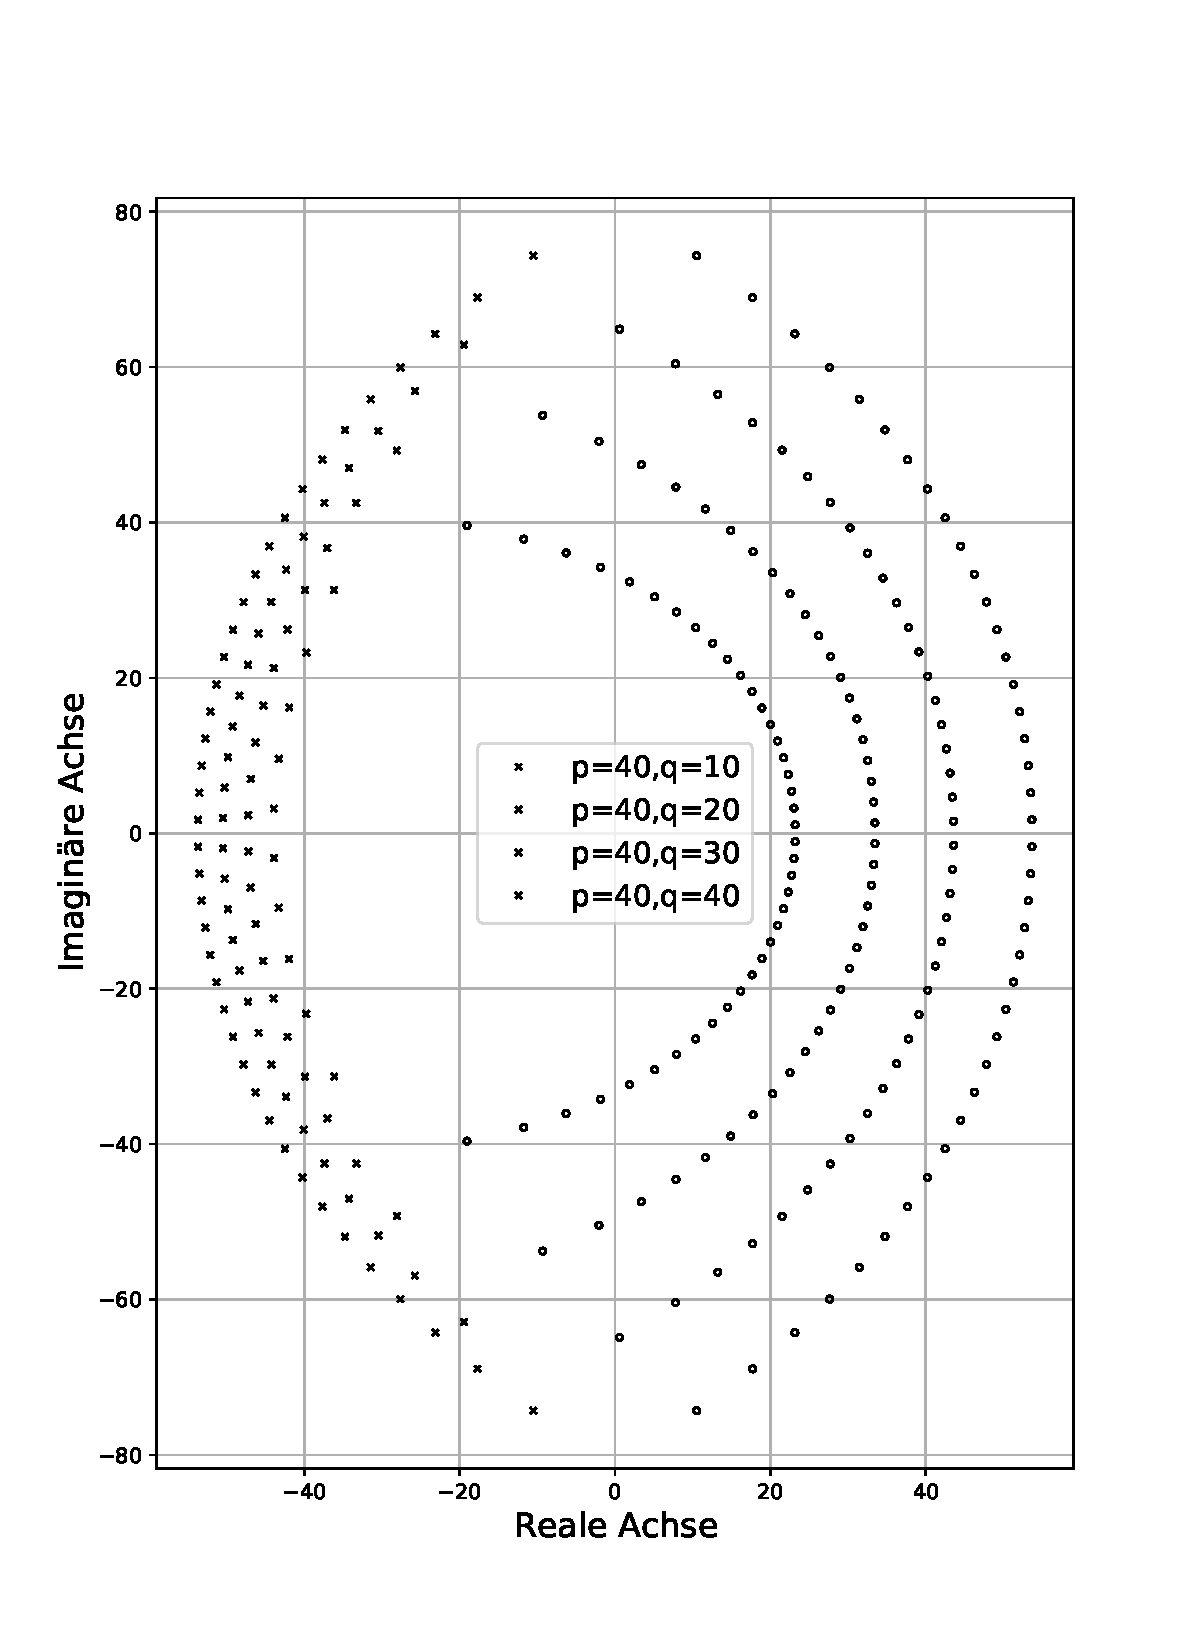
\includegraphics[width=0.45\linewidth]{./papers/pade/python/bilder/poles3.pdf}}
	\caption{Visualisierung der Stabilität der Padé-Polynome bei ungleicher $[L/M]$ Ordnung. \label{pade:prole}}
\end{figure}

\begin{figure}
	\centering
	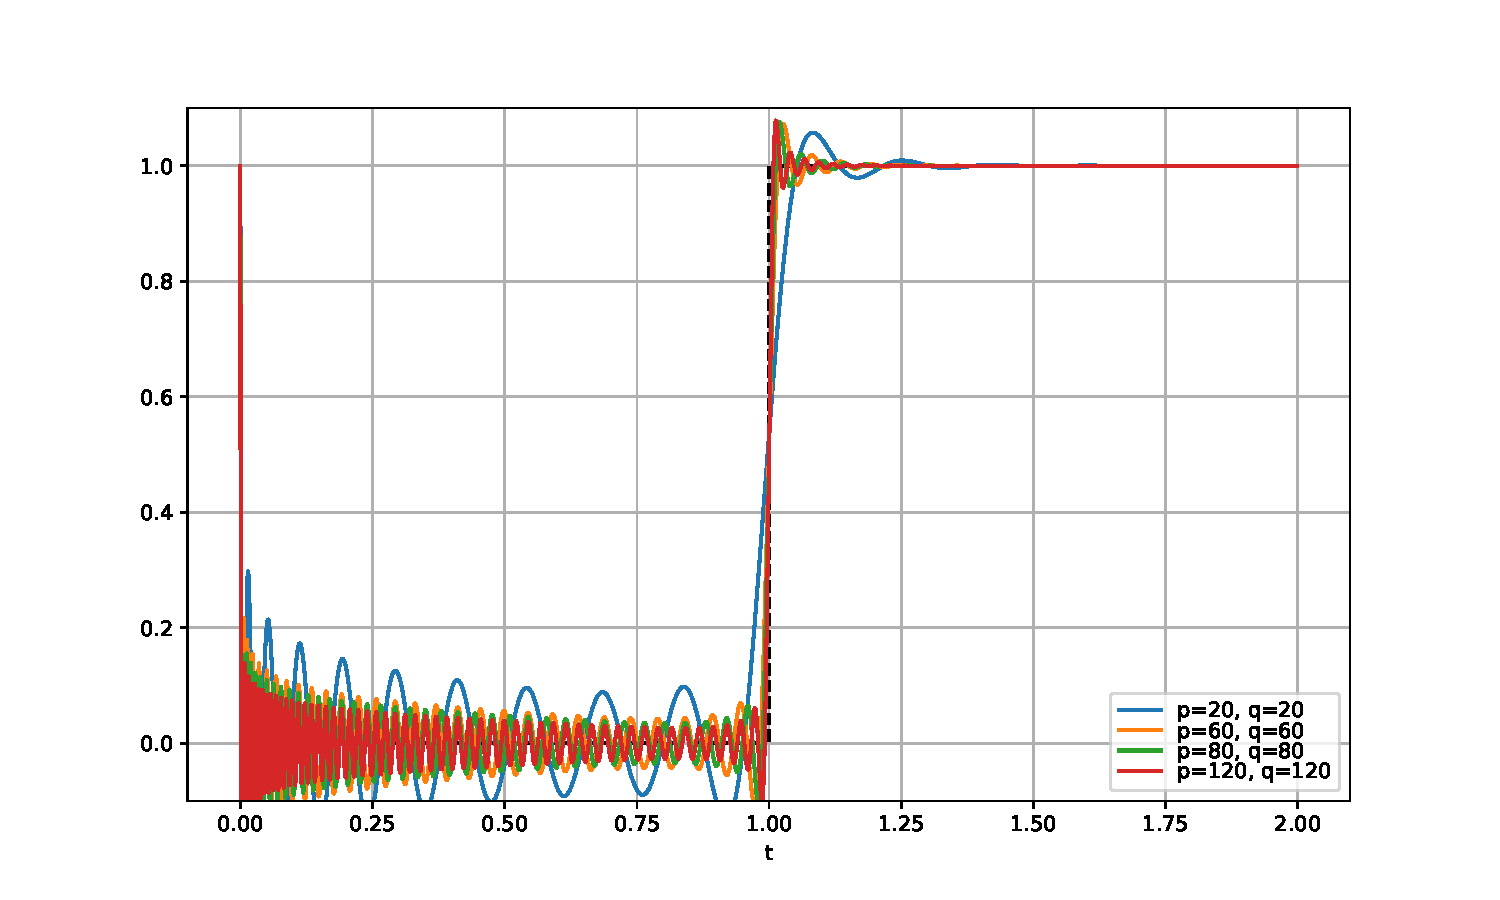
\includegraphics[width=1\linewidth]{./papers/pade/python/bilder/padehigh1.pdf}
	\caption{In den Zeitbereich zurück transformierte Polynome höherer Ordnungen \label{pade:totzeit}.}
\end{figure}

\todo{Abschluss welche Methoden bei der Rücktransformation nicht funktionieren und wie man das umgehen kann}


\subsection{Signal Modellierung
	\label{pade:subsection:SignalMod}}

Das Ziel einer Signalmodellierung ist dass eine parametrische Beschreibung eines Signales gefunden wird.
Dies kann für die Filterentwicklung, Interpolation, Extrapolation oder Kompression verwendet werden.
Dabei kann man immer das gleiche Modell verwenden, welches der Ausgang eines linearen verschiebungsinvarianten Filters zu einem Eingang $v(n)$ darstellt. 
\begin{figure}
	\centering
	\tikzset{>=latex}
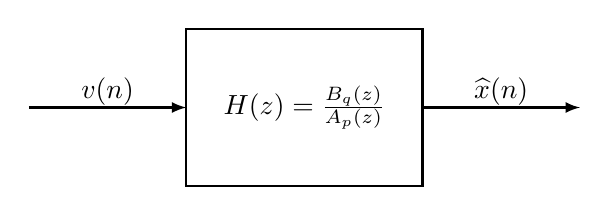
\begin{tikzpicture}
\node at (-1,1.2)  {$v(n)$}; 
\draw[thick,->] (-2,1)--(0,1);
\draw[thick] (0,0) rectangle (3,2) node[pos=.5] {$H(z)=\frac{B_q (z)}{A_p (z)}$};
\draw[thick,->] (3,1)--(5,1);
\node at (4,1.2)  {$\widehat{x}(n)$}; 
\end{tikzpicture}
\end{figure}
Dieses Modell wird mit

\begin{equation}
H(z)
=
\frac{B_{q}(z)}{A_{p}(z)}
=
\frac{\sum_{k=0}^{q} b_{q}(k) z^{-k}}{1+\sum_{k=1}^{p} a_{p}(k) z^{-k}}
\end{equation}
als eine rationale Funktion beschrieben.
Das Eingangssignal welches auf den Filter wirkt ist meist ein diskreter Impuls $\delta(n)$.
Der Modellierungsfehler setzt sich dabei aus der Einheitssprungantwort $h(n)$ und dem diskreten Signal $x(n)$ zusammen.
Dabei ist das Ziel den quadratischen Fehler (Least Squares Method)
\begin{equation}
\mathcal{E}_{L S}
=
\sum_{n=0}^{\infty}\left|e^{\prime}(n)\right|^{2}
\end{equation}
des Systems zu minimieren.
Um dies zu erreichen   
\begin{equation}\begin{array}{ll}
\frac{\partial \mathcal{E}_{L S}}{\partial a_{p}^{*}(k)}
=
0 
& 
; k=1,2, \ldots, p \\
\frac{\partial \mathcal{E}_{L S}}{\partial b_{q}^{*}(k)}
=
0 ; 
&
 k=0,1, \ldots, q
\end{array}\end{equation}
werden die Ableitungen gleich 0 gesetzt.
Aus diesen Bedienungen resultiert eine Menge von nichtlinearen Gleichungen 

\begin{equation}
\frac{\partial \mathcal{E}_{L S}}{\partial a_{p}^{*}(k)}
=
\frac{1}{2 \pi} 
\int_{-\pi}^{\pi}
\left[X\left(e^{j \omega}\right)-\frac{B_{q}\left(e^{j \omega}\right)}{A_{p}\left(e^{j \omega}\right)}\right] 
\frac{B_{q}^{*}\left(e^{j \omega}\right)}{\left[A_{p}^{*}\left(e^{j \omega}\right)\right]^{2}} 
e^{j k \omega} d \omega
=
0
\end{equation}
\begin{equation}
\frac{\partial \mathcal{E}_{L S}}{\partial b_{q}^{*}(k)}
=
-\frac{1}{2 \pi} 
\int_{-\pi}^{\pi}
\left[X\left(e^{j \omega}\right)-\frac{B_{q}\left(e^{j \omega}\right)}{A_{p}\left(e^{j \omega}\right)}\right] 
\frac{e^{j k \omega}}{A_{p}^{*}\left(e^{j \omega}\right)} d \omega
=
0
\end{equation}

\todo{Zitieren}

welche möglicherweise sehr schwierig lösbar sind.
Aus diesem Grund wird in der Praxis der Ansatz des kleinsten quadratischen Fehlers vermieden. 


\begin{figure}
	\centering
	\tikzset{>=latex}
	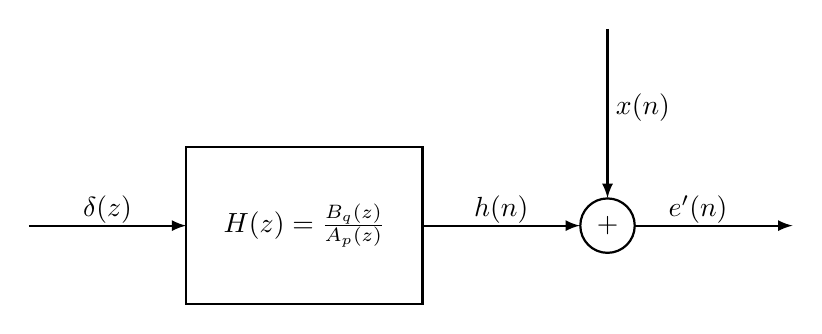
\begin{tikzpicture}
	\node at (-1,1.2)  {$\delta(z)$}; 
	\draw[thick,->] (-2,1)--(0,1);
	\draw[thick] (0,0) rectangle (3,2) node[pos=.5] {$H(z)=\frac{B_q (z)}{A_p (z)}$};
	\draw[thick,->] (3,1)--(5,1);
	\node [circle, draw, thick] at (5.35,1){+};
	\draw[thick,->] (5.35,3.5)--(5.35,1.35);
	\draw[thick,->] (5.7,1)--(7.7,1);
	\node at (4,1.2)  {$h(n)$}; 
	\node at (5.8,2.5)  {$x(n)$}; 
	\node at (6.5,1.2)  {$e^{\prime}(n)$}; 
	\end{tikzpicture}
\end{figure}

\todo{Beispiel Signal Modellierung mit Padé-Approximation Zeigen}

\todo{Folgerung schreiben}



